\documentclass[a4paper]{article}
\usepackage[utf8]{inputenc}
\usepackage{setspace}
\usepackage{graphicx}
\title{Criterion B: Analysis}
\date{May 2017}
\onehalfspacing
\begin{document}
\maketitle

\section*{Proposed solution}

Create a blog-based website with the ability to upload and download documents. The website will be built by using WordPress and back-end MySQL server. The website will be using Linux Hosting on my own machine that is 24/7 connected to the global net. 
\section*{Requirement specification}

\subsection*{IT system requirements}

\begin{itemize}
    \item Hardware - Personal Computer with Internet Connection, ARM Cortex-A53 x64 processor, 32 GB secondary storage, portable flash drive for backups.
    \item Software - Debian based Linux distribution, terminal, Google Chrome as the main web browser, Mozilla Firefox will be used as a second web browser to check the compatibility issues, Adobe Photoshop to create and edit images, Adobe Acrobat PDF Reader.
    \item Network - access to the Internet and required websites 
\end{itemize}

\subsection*{System interaction}

\begin{itemize}
    \item Complete full compatibility of edited images from Adobe Photoshop with WordPress integrated image editor.
    \item Back-end server MySQL, Adobe Photoshop, Google Chrome, Mozilla Firefox, Adobe Acrobat PDF Reader and Debian based Linux distribution is already installed on my system.
    \item Compatibility of website’s content and the back-end server.
    \item Ensure that website will work correctly on all popular supported web browsers, like Google Chrome, Mozilla Firefox, Internet Explorer, Microsoft Edge, Tor Web Browser, Opera Web Browser, and Yandex Open Browser.
\end{itemize}

\subsection*{Input/Output requirements}

\subsubsection*{Input requirements}

\begin{itemize}
    \item Information from Bulat Mukhamedievich as scientific publications, reports and articles.
    \item Client's own photos to add to a gallery.
    \item Client's biography information. Initially in Russian. Later translated into English by me. 
\end{itemize}

\subsubsection*{Output requirements}

\begin{itemize}
    \item Blog based website.
    \item Each page on the website will contain specific information and data.
    \item Every user should be able to open my client’s website and freely navigate through it.
    \item The design should be appropriate to client’s desires and format.
    \item Users should be able to leave comments on client’s pages. Comments will be moderated.
\end{itemize}

\subsection*{Processing}

\begin{itemize}
    \item Posting/editing client’s publications and articles on separate pages.
    \item Create a template for web pages, where new publication can be added easily.
    \item Upload original content on the website as edited images and translations.
\end{itemize}

\subsection*{Security}

\begin{itemize}
    \item The whole phpMyAdmin database will be backed up in the .sql file.
    \item Only me and the client will have accounts with administrative privileges.
    \item “Work in Progress” pages will be visible only to super users. (With administrative privileges)
\end{itemize}

\section*{Specific performance criteria}

The effectiveness of the website will be tested by these criteria's:

\begin{enumerate}
    \item A well-designed website.
    \item User-friendly design.
    \item Possibility to upload and download files as publications and articles.
    \item Open pages and be able to easily navigate between them.
    \item A regular automatic or manual backups.
    \item Possibility for guests and users to leave comments.
    \item Every source of data is reliable and content will be appropriate for visitation by various users.
\end{enumerate}

\section*{Justification of chosen solution}

The website most likely and the best way to share my client's works and scientific publications, so that any user across the globe can get an access to the content of the website. The websites structure – blog, makes it easier to add, edit and delete new blog posts, which may contain Bulat Mukhamediyev’s new scientific works and publications. Most important it is the needed software. My client would need only internet access and an appropriate web browser to access his website.\\

Below I will show how the proposed solution is meeting my client's specific requirements for a new IT system.

\begin{itemize}
  
\item Multiple software will be used only during the system development; after implementation, the system will be uploaded to a hosting website with their database.

\item I have already talked with my client multiple times. Bulat Mukhamediyev does agree that the website would be a great choice to spread his documents and to help young scientists/mathematicians. The WordPress is working on NGINX server with back-end server MySQL. NGINX server type is chosen because of its fast deployability and reliability. For example, in comparison with Apache Server, NGINX servers can handle more individual requests per short period of time.

\item The security features are also available. The MySQL server has the option to backup the selected database in different extensions. The screen can be seen in Figure \ref{fig:mysql}

\item The server that I am using to build and deploy the website is sufficient to the hardware and software requirements, which were introduced before.

\item All the equipment and software that I needed to develop and deploy the website are available. NGINX server software, Debian-based distribution - Raspbian, mysql back-end Database software and Wordpress are all free-to-use or open-sourced. The only expenses was the hardware of the system: server - Raspberry Pi 3 Model B (35\$), SD card (13\$) and other cables with converters (20\$).

\item Thanks to fast NGINX deployability features and Wordpress optimizations, I will be able to release the product (website) to the public within the time constraints.

\item Previously, I have had an experience on working with back-end databases, Linux hostings and website building. I have the required set of skills to realize the project.

\item As discussed in the Criterion A, my client sent me all the data and information that I needed for the website: biography information, articles/papers/publications and photos.

\item I am the only developer of the project. Simultaneously, I will be front-end and back-end developer. All the bugs and errors will be fixed and patched by me. The code of the project will remain non-open-source, until my client would not like to do otherwise.

\item All the costs and financial considerations will be taken care of by me. I will fund the project from the very beginning until its end. I will also cover all the maintenance costs.

\item The website will be password-protected, so no outside or third-party users will be able to access or change data without my or client's permission.

\item After the completion of the project, I will show my client how to operate the website on the level that he will need to be able to operate. For example: adding new pages, adding new posts and etc.

\item The only limitation in this IT system is the hardware used. The server is powerful enought to respond to tens of users simultaneously, but it is not powerful enough to provide access to hundreds of users. Under the heavy demand, server can crash. More powerful hardware can be used or a cloud server subscription can be used: AWS, BlueWhale, Azure, etc.

\item The WordPress Editor and the dashboard are working on the NGINX server, where all the data and information on the site is stored in mysql database. Figure \ref{fig:word} demonstrates the WordPress integrated dashboard.\\
  
\end{itemize}

\begin{figure}[h!]
    \centering
    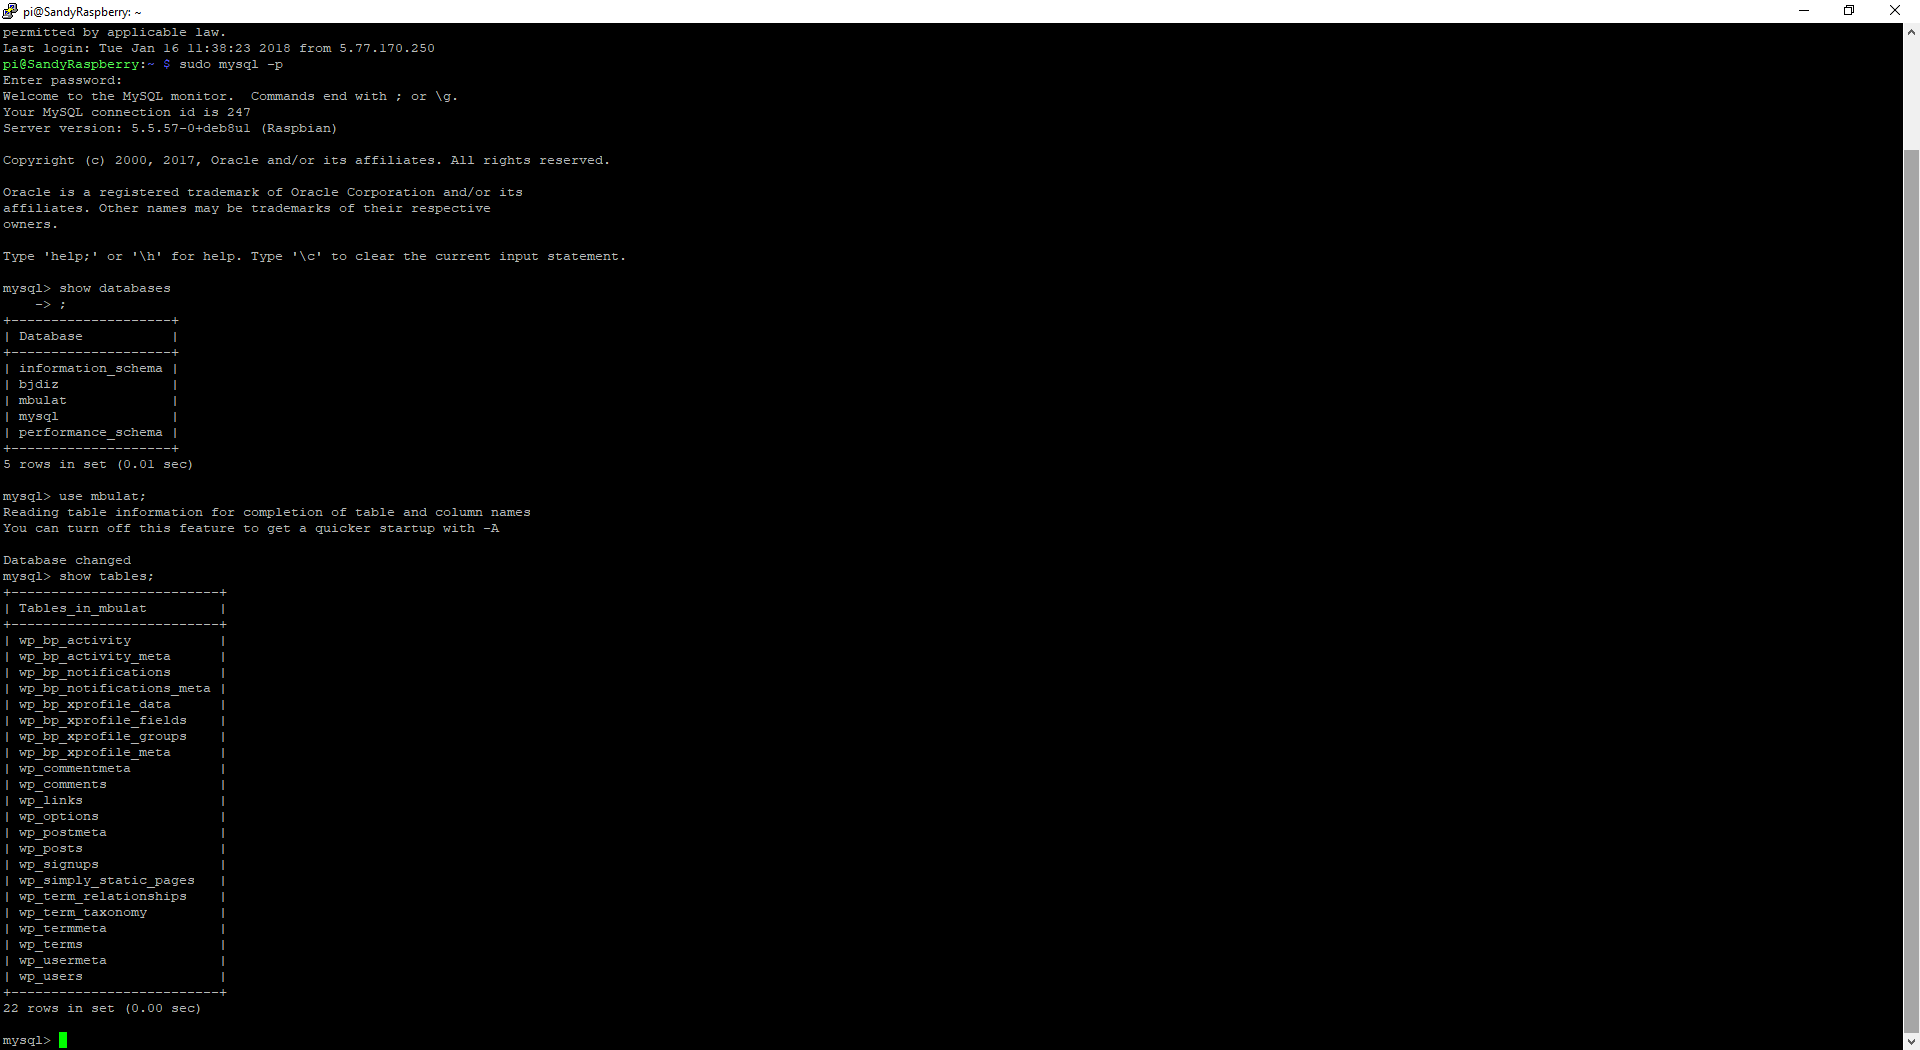
\includegraphics[width=\linewidth]{mysql.png}
    \caption{Screenshot of a mysql database from the terminal of the hosting machine}
    \label{fig:mysql}
\end{figure}

\begin{figure}[h!]
    \centering
    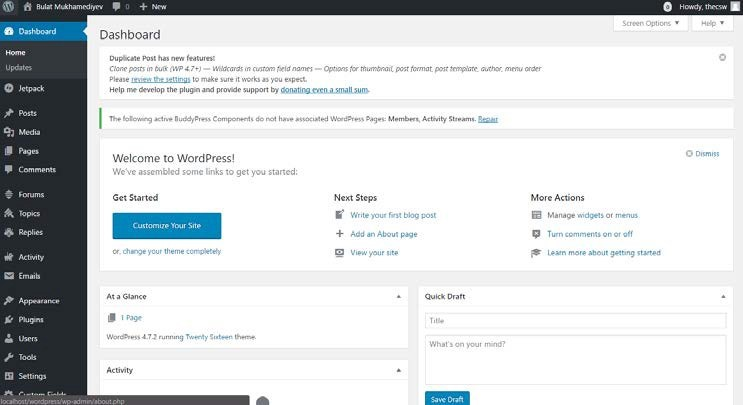
\includegraphics[width=\linewidth]{word.jpg}
    \caption{Screenshot of Wordpress dashboard}
    \label{fig:word}
\end{figure}

\end{document}
